\section{Customize}
%The customize window and widgets (spinner/colorpicker)
%\textit{Introduktion til customize fragmentet.\\
%Beskrivelse af arkitekturen i fragmentet\\
%Beskrivelse (med eksempler) af implementationen af de forskellige elementer (knapper osv.) i customize fragmentet}
The customize fragment is where the configurations are generated and altered.\\
\\
As stated in \autoref{cha:analysis} the timers our contact person use has different sizes and colors, these customization options are essential for the timer application.
The list of customization features are as follows:

\begin{itemize}
	\item Change style of the timer.
	\item Change the timespan of the timer.
	\item Change the color of the timer and background.
	\item Change the color of the timer to be changing gradiently.
	\item Attach one or two pictograms, or a timer.
	\item Change the default done pictogram to one or two pictograms.
	\item Save the timer.
	\item Start the timer.
\end{itemize}

\subsection{Architecture of Customize}
\label{subsec:cust_arch}
The customize fragment consists of four main elements, the first element is the style picker where the user can change the style of the timer.
The second element is the time wheels where the user can change the timespan of the timer.
The third element is the color pickers where the user can change the colors of the time left, the frame, and the background of the timer.
The fourth element is the menu where the modifications like attachment is found.
Figure \ref{fig:customize:layout} show architecture of the fragment.

\begin{figure}[H]
	\centering
		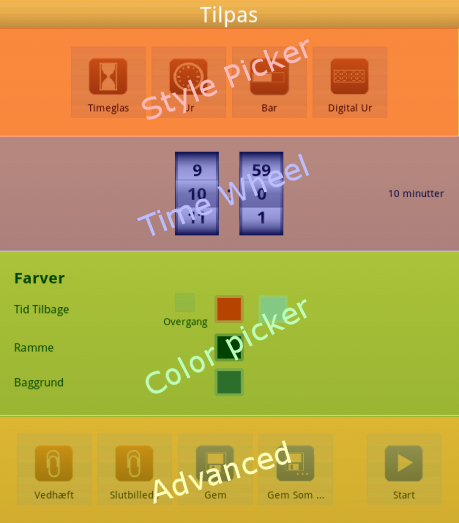
\includegraphics[width=0.5\textwidth]{Images/Implementation/customize_layout.png}
	\caption{An outline of the architecture of the customize fragment.}
	\label{fig:customize:layout}
\end{figure}

All functionality of the items in the customize fragment in placed in the customize class.
For further development a refactoring of the entire class is advised such that all buttons in WOMBAT is handled like the \texttt{WDialog}, which can be found in \autoref{subsubsec:attach}.

To be able to get an overview of the items in the customize fragment all items are assigned a method, these methods are then referenced from the \texttt{onCreate} method in \autoref{code:customize:oncreate}. An example of one of these methods is the style chooser in \autoref{code:customize:style_choser}.

\begin{figure}[H]
\begin{lstlisting}
public void onActivityCreated(Bundle savedInstanceState) {
	super.onActivityCreated(savedInstanceState);
	currSubP = new SubProfile("", "", 0xff3D3D3D, 0xffFF0000, 0xffB8B8B8,
			0xff000000, 600, false);
	currSubP.save = false;
	currSubP.saveAs = false;

	/********* TIME CHOSER *********/
	initStyleChoser();

...

	/******** BOTTOM MENU ***********/
	initBottomMenu();
}
\end{lstlisting}
\caption{The \texttt{onCreate} method, which calls the button initializers in the same order as they are shown in the layout.}%
\label{code:customize:oncreate}%
\end{figure}


\begin{figure}[H]
\begin{lstlisting}
private void initStyleChoser() {
	hourglassButton = (Button) getActivity().findViewById(
			R.id.houglassButton);
	hourglassButton.setOnClickListener(new OnClickListener() {

		public void onClick(View v) {
			selectStyle(formFactor.Hourglass);
		}
	});

	timetimerButton = (Button) getActivity().findViewById(
			R.id.timetimerButton);
	timetimerButton.setOnClickListener(new OnClickListener() {

		public void onClick(View v) {
			selectStyle(formFactor.TimeTimer);
		}
	});

	progressbarButton = (Button) getActivity().findViewById(
			R.id.progressbarButton);
...
\end{lstlisting}
\caption{The style chooser initialization method, which utilize the \texttt{selectStyle} that changes the style of the timer and highlights the button.}%
\label{code:customize:style_choser}%
\end{figure}

\subsection*{Buttons in Customize}
There is four kinds of buttons in the customize fragment:

\begin{itemize}
	\item Start, save, and style buttons.
	\item Time picker wheels.
	\item Color picker.
	\item Attachment and done pictogram button.
\end{itemize}

\subsubsection*{Start Button}
The style, save, start, and attachment buttons are default Android buttons with a picture attached on top.
The differences of these buttons is the \texttt{onClick} event handler, figure \ref{code:customize:start_button} is the source code of the start button.

\begin{figure}[H]
\begin{lstlisting}
private void initStartButton() {
 startButton = (Button) getActivity().findViewById(
		 R.id.customize_start_button);
 Drawable d;
 if (currSubP.saveAs) {
	 d = getResources().getDrawable(R.drawable.thumbnail_start);
	 startButton.setOnClickListener(new OnClickListener() {

		 public void onClick(View v) {
			 currSubP.addLastUsed(preSubP);
			 guard.saveGuardian(currSubP);
			 currSubP.select();
			 Intent i = new Intent(
					 getActivity().getApplicationContext(),
					 DrawLibActivity.class);
			 startActivity(i);
		 }
	 });
 } else {
				...
		 }
	 });
 }

 startButton
 .setCompoundDrawablesWithIntrinsicBounds(null, d, null, null);
}
\end{lstlisting}
\caption{The source code of the start button, which sets the top image of the button to the drawable \texttt{thumbnail\_start\_gray}}%
\label{code:customize:start_button}%
\end{figure}

\subsubsection*{Time Picker Wheels}
The time picker is a widget\cite{web:android:customize:wheel}.
All functionality of the wheel widget is handled by the widget itself and only requires the widget to be imported to Eclipse and added as a project library, which is a built-in feature in the Android development environment.

WOMBAT is limited to timers on 60 minutes, therefore we implement a functionality which sets the seconds wheel to zero whenever the minutes wheel is set to 60, this can be seen in figure \ref{code:customize:time_picker_wheels}.

\begin{figure}[H]
\begin{lstlisting}
private int previousMins;
private int previousSecs;
private void initTimePicker() {
	/* Create minute Wheel */
	mins = (WheelView) getActivity().findViewById(R.id.minPicker);
	mins.setViewAdapter(new NumericWheelAdapter(getActivity()
			.getApplicationContext(), 0, 60));
	mins.setCyclic(true);

	/* Add on change listeners for both wheels */
	mins.addChangingListener(new OnWheelChangedListener() {
		public void onChanged(WheelView wheel, int oldValue, int newValue) {
			updateTime(mins.getCurrentItem(), secs.getCurrentItem());

			if (mins.getCurrentItem() == 60) {
				previousMins = 60;
				previousSecs = secs.getCurrentItem();

				secs.setCurrentItem(0);
				secs.setViewAdapter(new NumericWheelAdapter(getActivity()
						.getApplicationContext(), 0, 0));
				secs.setCyclic(false);
			} else if (previousMins == 60) {
				secs.setViewAdapter(new NumericWheelAdapter(getActivity()
						.getApplicationContext(), 0, 60));

				secs.setCurrentItem(previousSecs);
				secs.setCyclic(true);
				previousMins = 0;
			}
		}
	});
}
\end{lstlisting}
\caption{The time picker wheels.}%
\label{code:customize:time_picker_wheels}%
\end{figure}


\subsubsection*{Color Picker}
Just like the time picker wheels we utilize the widget functionality in Android to implement a widget called AmbilWarna\footnote{AmbilWarna means "Take Color" in Indonesian}, to handle the color picker\cite{web:android:customize:color}.
The color picker widget is a custom dialog which returns the color picked by the user in the widget, the implementation of the color picker widget can be found in \autoref{code:customize:color_picker}.
\begin{figure}[H]
\begin{lstlisting}
colorGradientButton2 = (Button) getActivity().findViewById(
		R.id.gradientButton_2);
setColor(colorGradientButton2.getBackground(), currSubP.timeSpentColor);
colorGradientButton2.setOnClickListener(new OnClickListener() {
	public void onClick(View v) {
		AmbilWarnaDialog dialog = new AmbilWarnaDialog(getActivity(),
				currSubP.timeSpentColor, new OnAmbilWarnaListener() {
			public void onCancel(AmbilWarnaDialog dialog) {
			}

			public void onOk(AmbilWarnaDialog dialog, int color) {
				currSubP.timeSpentColor = color;
				setColor(colorGradientButton2.getBackground(),
						currSubP.timeSpentColor);
			}
		});
		dialog.show();
	}
});
\end{lstlisting}
\caption{The color picker widget implemented on the second "Time Left" color button}%
\label{code:customize:color_picker}%
\end{figure}

\subsubsection*{Attachment Button}
\label{subsubsec:attach}
The attachment buttons are implemented like the start button, the difference is that they make use of a custom dialog in WOMBAT.
This custom dialog, \texttt{WDialog}, is created because the standard dialogs in Android are very different from the rest of the WOMBAT design.
Also the standard dialogs limit the programmer to use exactly the buttons defined in the dialog API.\\
The custom dialog is implemented because the standard dialogs are inconsistent with the WOMBAT design and the custom dialogs are much more versatile when adding buttons.
Figure \ref{code:customize:wdialog} is an example of how a dialog could be specified.

\begin{figure}[H]
\begin{lstlisting}
final WDialog attachment1 = new WDialog(getActivity(),
	R.string.attachment_dialog_description);

ModeAdapter adapter = new ModeAdapter(getActivity(),
	android.R.layout.simple_list_item_1, mode);

attachment1.setAdapter(adapter);

attachment1.addButton(R.string.cancel, 1,
	new OnClickListener() {

	public void onClick(View arg0) {
		attachment1.cancel();
	}
});
\end{lstlisting}
\caption{Initialization of the dialog, that appears when the attachment button is clicked, the \texttt{OnItemClickListener} is not shown here because of lack of space on the page.}%
\label{code:customize:wdialog}%
\end{figure}